% Practice Test 12 — Minnesota Edition
% Questions: 30 (17 MC + 13 SA)
% Generated by scripts/generate_practice_tests.py

\begin{practiceQuestion}{1-3-q20}{sa}
\begin{questionText}
A store sells ribbon at a constant price per yard. If $3$ yards cost $\$4.50$, what is the constant of proportionality?
\end{questionText}
\correctAnswer{$k = \$1.50$ per yard}
\explanation{$k = \frac{4.50}{3} = 1.50$ dollars per yard.}
\end{practiceQuestion}

\begin{practiceQuestion}{1-5-q20}{sa}
\begin{questionText}
Two delivery services are proportional. Service A: $(2, 14)$. Service B: $(3, 18)$. Which has the higher rate and what is it?
\end{questionText}
\correctAnswer{Service A at $\$7$ per delivery}
\explanation{Service A: $k = \frac{14}{2} = 7$. Service B: $k = \frac{18}{3} = 6$. Service A has the higher rate at $\$7$.}
\end{practiceQuestion}

\begin{practiceQuestion}{1-6-q19}{sa}
\begin{questionText}
A recipe for $6$ servings uses $\frac{3}{4}$ cup of sugar. How much sugar is needed for $16$ servings?
\end{questionText}
\correctAnswer{$2$ cups}
\explanation{Per serving: $\frac{3}{4} \div 6 = \frac{3}{24} = \frac{1}{8}$ cup. For $16$: $\frac{1}{8} \times 16 = 2$ cups.}
\end{practiceQuestion}

\begin{practiceQuestion}{2-1-q21}{sa}
\begin{questionText}
$56$ is $80\%$ of what number?
\end{questionText}
\correctAnswer{$70$}
\explanation{Divide: $56 \div 0.80 = 70$.}
\end{practiceQuestion}

\begin{practiceQuestion}{2-5-q10}{mc}
\begin{questionText}
A car salesperson earns $4\%$ commission. She sold a car for $\$28{,}000$. How much commission did she earn?
\end{questionText}
\choiceA{$\$700$}
\choiceB{$\$1{,}120$}
\choiceC{$\$2{,}800$}
\choiceD{$\$11{,}200$}
\correctAnswer{B}
\explanation{$28{,}000 \times 0.04 = \$1{,}120$.}
\end{practiceQuestion}

\begin{practiceQuestion}{2-7-q29}{gsa}
\begin{questionText}
The table shows the results of a science experiment. Calculate the percent error for Trial 3 (round to the nearest tenth).

\begin{center}
\begin{tabular}{|l|c|c|c|}
\hline
 & \textbf{Predicted (g)} & \textbf{Actual (g)} & \textbf{Percent Error} \\
\hline
Trial 1 & $50$ & $48$ & $4.2\%$ \\
\hline
Trial 2 & $50$ & $55$ & $9.1\%$ \\
\hline
Trial 3 & $50$ & $44$ & ? \\
\hline
\end{tabular}
\end{center}
\end{questionText}
\correctAnswer{$\approx 13.6\%$}
\explanation{$\frac{|50 - 44|}{44} \times 100 = \frac{6}{44} \times 100 \approx 13.6\%$.}
\end{practiceQuestion}

\begin{practiceQuestion}{2-8-q23}{sa}
\begin{questionText}
Name one advantage and one disadvantage of using a credit card instead of a debit card.
\end{questionText}
\correctAnswer{Advantage: buy now, pay later; Disadvantage: you may pay interest}
\explanation{Credit cards let you purchase before having the cash, but you owe interest if you don't pay the full balance on time.}
\end{practiceQuestion}

\begin{practiceQuestion}{3-1-q27}{gmc}
\begin{questionText}
The number line below shows two points. Which statement is correct?

\begin{center}
\begin{tikzpicture}
  \draw[thick,->] (-6.5,0) -- (6.5,0);
  \foreach \x in {-6,...,6} \draw (\x,0.1) -- (\x,-0.1) node[below] {$\x$};
  \fill[funBlue] (-4,0) circle (4pt) node[above=6pt] {P};
  \fill[funBlue] (4,0) circle (4pt) node[above=6pt] {Q};
\end{tikzpicture}
\end{center}
\end{questionText}
\choiceA{P and Q are the same number}
\choiceB{P and Q are opposites}
\choiceC{$|P| > |Q|$}
\choiceD{$P > Q$}
\correctAnswer{B}
\explanation{Point P is at $-4$ and Q is at $4$. They are the same distance from $0$ on opposite sides, so they are opposites.}
\end{practiceQuestion}

\begin{practiceQuestion}{4-1-q20}{sa}
\begin{questionText}
Evaluate $-3x + 14$ when $x = -5$.
\end{questionText}
\correctAnswer{$29$}
\explanation{Substitute: $-3(-5) + 14 = 15 + 14 = 29$.}
\end{practiceQuestion}

\begin{practiceQuestion}{4-2-q10}{mc}
\begin{questionText}
Simplify $2.5a + 1.3 - 0.5a + 2.7$.
\end{questionText}
\choiceA{$2a + 4$}
\choiceB{$3a + 4$}
\choiceC{$2a - 4$}
\choiceD{$6$}
\correctAnswer{A}
\explanation{Combine variable terms: $2.5a - 0.5a = 2a$. Combine constants: $1.3 + 2.7 = 4$. Result: $2a + 4$.}
\end{practiceQuestion}

\begin{practiceQuestion}{5-2-q24}{sa}
\begin{questionText}
Solve $\dfrac{k}{8} + 9 = 15$.
\end{questionText}
\correctAnswer{$k = 48$}
\explanation{Subtract $9$: $\frac{k}{8} = 6$. Multiply by $8$: $k = 48$. Check: $\frac{48}{8} + 9 = 6 + 9 = 15$ \checkmark.}
\end{practiceQuestion}

\begin{practiceQuestion}{5-3-q15}{mc}
\begin{questionText}
Three friends split the cost of a gift equally. Each person also pays $\$4$ for wrapping. Each person pays $\$16$ total. What is the cost $c$ of the gift?
\end{questionText}
\choiceA{$c = 48$}
\choiceB{$c = 36$}
\choiceC{$c = 12$}
\choiceD{$c = 60$}
\correctAnswer{B}
\explanation{Each pays $\frac{c}{3} + 4 = 16$. This means $\frac{c}{3} = 12$, so $c = 36$. Or: total paid $= 3 \times 16 = 48$, wrapping $= 3 \times 4 = 12$, gift $= 48 - 12 = 36$.}
\end{practiceQuestion}

\begin{practiceQuestion}{5-4-q03}{mc}
\begin{questionText}
Solve $0.25n - 1.5 = 3.5$.
\end{questionText}
\choiceA{$n = 8$}
\choiceB{$n = 20$}
\choiceC{$n = 14$}
\choiceD{$n = 2$}
\correctAnswer{B}
\explanation{Add $1.5$: $0.25n = 5$. Divide by $0.25$: $n = 20$. Check: $0.25(20) - 1.5 = 5 - 1.5 = 3.5$ \checkmark.}
\end{practiceQuestion}

\begin{practiceQuestion}{5-5-q16}{mc}
\begin{questionText}
Solve $\dfrac{n}{5} - 2 > 4$.
\end{questionText}
\choiceA{$n > 10$}
\choiceB{$n > 30$}
\choiceC{$n > 1$}
\choiceD{$n < 30$}
\correctAnswer{B}
\explanation{Add $2$: $\frac{n}{5} > 6$. Multiply by $5$: $n > 30$.}
\end{practiceQuestion}

\begin{practiceQuestion}{5-6-q09}{mc}
\begin{questionText}
A parking garage charges $\$5$ per hour. You have $\$30$. Which inequality represents the hours $h$ you can park, and what does the graph look like?
\end{questionText}
\choiceA{$5h \leq 30$; closed circle at $6$, shade left from $0$ to $6$}
\choiceB{$5h < 30$; open circle at $6$, shade left}
\choiceC{$5h \geq 30$; closed circle at $6$, shade right}
\choiceD{$5h > 30$; open circle at $6$, shade right}
\correctAnswer{A}
\explanation{You can spend at most $\$30$: $5h \leq 30$, so $h \leq 6$. Closed circle at $6$, shade left (and $h \geq 0$).}
\end{practiceQuestion}

\begin{practiceQuestion}{6-3-q27}{gmc}
\begin{questionText}
The diagram shows a triangle with the given measurements. How many different triangles can be drawn with these exact conditions?

\begin{center}
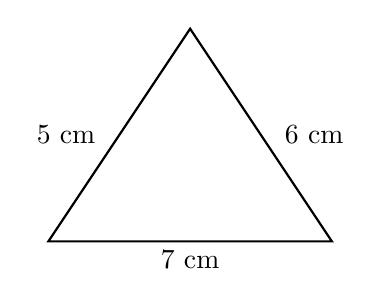
\begin{tikzpicture}[scale=0.9]
  \draw[thick] (0,0) -- (4,0) -- (2,3) -- cycle;
  \node[below] at (2,0) {$7$ cm};
  \node[left] at (0.8,1.5) {$5$ cm};
  \node[right] at (3.2,1.5) {$6$ cm};
\end{tikzpicture}
\end{center}
\end{questionText}
\choiceA{None}
\choiceB{Exactly one}
\choiceC{Exactly two}
\choiceD{Infinitely many}
\correctAnswer{B}
\explanation{Three side lengths that satisfy the triangle inequality (SSS) produce exactly one unique triangle. Check: $5 + 6 = 11 > 7$, $5 + 7 = 12 > 6$, $6 + 7 = 13 > 5$. All pass.}
\end{practiceQuestion}

\begin{practiceQuestion}{6-4-q15}{mc}
\begin{questionText}
You know two angles of a triangle are $55°$ and $65°$ and a non-included side is $9$ cm. This is an example of:
\end{questionText}
\choiceA{SSS}
\choiceB{SAS}
\choiceC{ASA}
\choiceD{AAS}
\correctAnswer{D}
\explanation{Two angles and a non-included side is AAS (Angle-Angle-Side). This produces a unique triangle.}
\end{practiceQuestion}

\begin{practiceQuestion}{6-5-q02}{mc}
\begin{questionText}
You slice a cylinder with a horizontal cut parallel to its base. What shape is the cross-section?
\end{questionText}
\choiceA{Rectangle}
\choiceB{Circle}
\choiceC{Oval}
\choiceD{Triangle}
\correctAnswer{B}
\explanation{A horizontal cut through a cylinder parallel to the circular base produces a circle.}
\end{practiceQuestion}

\begin{practiceQuestion}{6-6-q23}{sa}
\begin{questionText}
An angle is $3$ times its complement. Find the angle.
\end{questionText}
\correctAnswer{$67.5°$}
\explanation{Let complement be $x$. Angle $= 3x$. Sum: $x + 3x = 90$. So $4x = 90$ and $x = 22.5°$. The angle: $3(22.5) = 67.5°$.}
\end{practiceQuestion}

\begin{practiceQuestion}{7-3-q24}{sa}
\begin{questionText}
A circular plate has a diameter of $28$ cm. What is its area? Use $\pi \approx \frac{22}{7}$.
\end{questionText}
\correctAnswer{$616$ cm$^2$}
\explanation{$r = 14$ cm. $A = \frac{22}{7} \times 196 = 616$ cm$^2$.}
\end{practiceQuestion}

\begin{practiceQuestion}{7-4-q28}{gmc}
\begin{questionText}
The diagram shows a figure made of a rectangle and a triangle. What is the total area?

\begin{center}
\begin{tikzpicture}[scale=0.5]
  \fill[funBlue!20] (0,0) -- (10,0) -- (10,4) -- (5,7) -- (0,4) -- cycle;
  \draw[thick,funBlue] (0,0) -- (10,0) -- (10,4) -- (5,7) -- (0,4) -- cycle;
  \draw[dashed,gray] (0,4) -- (10,4);
  \draw[thick,funRed,<->] (0,-0.7) -- (10,-0.7);
  \node[below,funRed] at (5,-0.7) {$10$ m};
  \draw[thick,funRed,<->] (10.7,0) -- (10.7,4);
  \node[right,funRed] at (10.7,2) {$4$ m};
  \draw[thick,funRed,<->] (5,4) -- (5,7);
  \node[right,funRed] at (5,5.5) {$3$ m};
\end{tikzpicture}
\end{center}
\end{questionText}
\choiceA{$40$ m$^2$}
\choiceB{$55$ m$^2$}
\choiceC{$70$ m$^2$}
\choiceD{$85$ m$^2$}
\correctAnswer{B}
\explanation{Rectangle: $10 \times 4 = 40$ m$^2$. Triangle: $\frac{1}{2} \times 10 \times 3 = 15$ m$^2$. Total: $40 + 15 = 55$ m$^2$.}
\end{practiceQuestion}

\begin{practiceQuestion}{7-5-q05}{mc}
\begin{questionText}
A cube has a surface area of $150$ cm$^2$. What is the side length of the cube?
\end{questionText}
\choiceA{$5$ cm}
\choiceB{$10$ cm}
\choiceC{$25$ cm}
\choiceD{$15$ cm}
\correctAnswer{A}
\explanation{$SA = 6s^2$. So $s^2 = 150 \div 6 = 25$. Therefore $s = 5$ cm.}
\end{practiceQuestion}

\begin{practiceQuestion}{7-6-q30}{gsa}
\begin{questionText}
A rectangular prism-shaped fish tank is shown below. If water fills the tank to $\frac{3}{4}$ of its height, what is the volume of water in the tank?

\begin{center}
\begin{tikzpicture}[scale=0.35]
  % Tank outline
  \draw[thick,funBlue] (0,0) rectangle (10,8);
  \draw[thick,funBlue] (10,0) -- (14,3) -- (14,11) -- (10,8);
  \draw[thick,funBlue] (0,8) -- (4,11) -- (14,11);
  % Water level at 3/4
  \fill[cyan!30] (0,0) rectangle (10,6);
  \fill[cyan!20] (10,0) -- (14,3) -- (14,9) -- (10,6) -- cycle;
  \draw[dashed,funRed] (0,6) -- (10,6) -- (14,9);
  \node[left,funRed] at (0,6) {water};
  % Labels
  \draw[thick,funRed,<->] (0,-0.8) -- (10,-0.8);
  \node[below,funRed] at (5,-0.8) {$20$ cm};
  \draw[thick,funRed,<->] (-1,0) -- (-1,8);
  \node[left,funRed] at (-1,4) {$16$ cm};
  \draw[thick,funRed,<->] (14.5,3) -- (14.5,11);
  \node[right,funRed] at (14.5,7) {$16$ cm};
  \node[below right,funRed] at (12,1.5) {$10$ cm};
\end{tikzpicture}
\end{center}
\end{questionText}
\correctAnswer{$2{,}400$ cm$^3$}
\explanation{Full tank volume: $20 \times 10 \times 16 = 3{,}200$ cm$^3$. Water at $\frac{3}{4}$ height: $20 \times 10 \times 12 = 2{,}400$ cm$^3$.}
\end{practiceQuestion}

\begin{practiceQuestion}{8-1-q17}{mc}
\begin{questionText}
A doctor wants to study the effect of a new medicine on $10{,}000$ patients. She randomly selects $500$ patients for a trial. What is the sample size?
\end{questionText}
\choiceA{$10{,}000$}
\choiceB{$500$}
\choiceC{$10{,}500$}
\choiceD{$50$}
\correctAnswer{B}
\explanation{The sample size is the number of individuals selected — $500$ patients.}
\end{practiceQuestion}

\begin{practiceQuestion}{8-3-q07}{mc}
\begin{questionText}
Two box plots are drawn on the same number line. Box plot A is entirely to the right of box plot B. What does this tell you?
\end{questionText}
\choiceA{Group A has more data}
\choiceB{All values in Group A are greater than all values in Group B}
\choiceC{Group A has no overlap with Group B}
\choiceD{Both B and C}
\correctAnswer{D}
\explanation{If box plot A is entirely to the right, every value in A exceeds every value in B, so there is no overlap.}
\end{practiceQuestion}

\begin{practiceQuestion}{8-4-q03}{mc}
\begin{questionText}
Group A has a mean of $50$ and a MAD of $3$. Group B has a mean of $60$ and a MAD of $3$. The difference in means expressed in MADs is:
\end{questionText}
\choiceA{$\frac{10}{3} \approx 3.3$ MADs}
\choiceB{$10$ MADs}
\choiceC{$3$ MADs}
\choiceD{$30$ MADs}
\correctAnswer{A}
\explanation{Difference $= 60 - 50 = 10$. In MADs: $\frac{10}{3} \approx 3.3$.}
\end{practiceQuestion}

\begin{practiceQuestion}{8-6-q21}{sa}
\begin{questionText}
A circle graph shows a budget of $\$2{,}000$. The housing sector is $40\%$. How much is spent on housing?
\end{questionText}
\correctAnswer{$\$800$}
\explanation{$40\%$ of $\$2{,}000 = 0.40 \times 2{,}000 = \$800$.}
\end{practiceQuestion}

\begin{practiceQuestion}{9-4-q15}{mc}
\begin{questionText}
Which of these is NOT a valid probability model?
\end{questionText}
\choiceA{$P(A) = 0.5$, $P(B) = 0.5$}
\choiceB{$P(A) = 0.7$, $P(B) = 0.2$, $P(C) = 0.1$}
\choiceC{$P(A) = 0.6$, $P(B) = 0.6$}
\choiceD{$P(A) = 1$}
\correctAnswer{C}
\explanation{$0.6 + 0.6 = 1.2 > 1$. The probabilities must sum to exactly $1$.}
\end{practiceQuestion}

\begin{practiceQuestion}{9-6-q25}{sa}
\begin{questionText}
Three coins are flipped. What is the probability of getting exactly $1$ head? Write your answer as a fraction in simplest form.
\end{questionText}
\correctAnswer{$\frac{3}{8}$}
\explanation{Outcomes with exactly $1$ head: HTT, THT, TTH — that is $3$ out of $8$. $P = \frac{3}{8}$.}
\end{practiceQuestion}

\begin{practiceQuestion}{9-7-q14}{mc}
\begin{questionText}
Mia uses a random number generator to produce digits $0$--$9$. She runs $20$ trials to simulate a $40\%$ chance of an event. In her simulation, the event happens $10$ times. What is the experimental probability?
\end{questionText}
\choiceA{$0.20$}
\choiceB{$0.40$}
\choiceC{$0.50$}
\choiceD{$0.10$}
\correctAnswer{C}
\explanation{$P = \frac{10}{20} = 0.50$. This is higher than the theoretical $0.40$, but with only $20$ trials, variation is expected.}
\end{practiceQuestion}
